\documentclass[a4paper,11pt,twoside]{article}
\usepackage[left=2.5cm,right=2cm,top=2cm,bottom=2cm]{geometry}

\usepackage{multirow}
\usepackage[table,xcdraw]{xcolor}
\usepackage{graphicx}
\usepackage{booktabs}
\usepackage{rotating}
\usepackage{epsfig}
\usepackage{amssymb}
\usepackage{amsmath}
\usepackage{amsfonts}
\usepackage{amsthm}
\usepackage{amsmath}
\usepackage{mathtools}
\usepackage{hyperref}
\usepackage{float}


\newcommand{\HRule}{\rule{\linewidth}{0.4mm}}

\setlength{\parindent}{0em}
\setlength{\parskip}{0.5em}

\begin{document}
\begin{center}
  \textbf{\LARGE Inferring Infection Times using Serological Data}\\[.5cm]
  \textbf{\Large Initial Simulation Results}\\[.5cm]
\end{center}

\section{Motivation}
There is a lot of information in the FluScape serological data that might be used to infer infections by both human and non-human influenza strains. We have HAI titres against a panel of strains at two time points, where boosting of antibody levels from sample one to sample two should be indicative of infection. However, simply using a 4-fold rise as an indicator of infection (seroconversion) might miss small boosts, not account for measurement error or miss cross-reactive boosting. 

We attempt to address these issues by combining data from the FluScape serological survey with a descriptive model of antibody kinetics. Our model has previously been used to describe antibody kinetics in a cohort of ferrets with known, varied exposure histories. By fitting this model using a Bayesian framework, we hope to estimate infection times for each individual in the presence of measurement error and multiple co-circulating strains. Although the FluScape data is only loosely longitudinal, covering just two time points, we hope to utilise the information present in the cross-sectional panel of tested strains.

This document provides a summary of the work done to date. In particular, we have defined a data-generating process to simulate a sero-survey like that of FluScape, and then use an MCMC approach to infer [known] infection times for each individual in the simulation.

\section{Simulation Description}
\subsection{Model}
\begin{figure}[h!]
\begin{center}
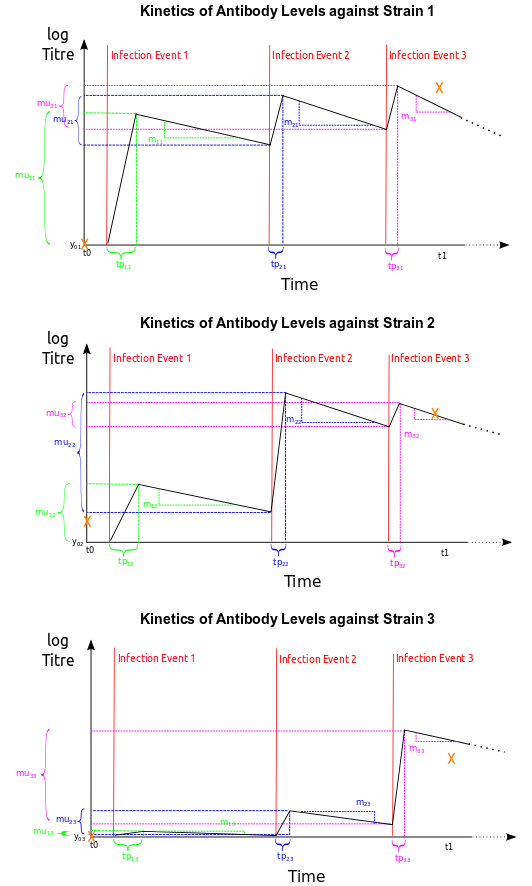
\includegraphics[scale=0.7]{model_cartoon.png}\\
\caption{Cartoon representation of the multiple-infection boosting/waning model. Vertical red lines represent times of infection events; orange crosses represent titre readings; other parameters are as described in the below text.}
\end{center}
\end{figure}
Figure 1 provides a cartoon representation of the model. For each individual, we are concerned with the kinetics of antibodies produced against each strain over the study period. We assume that each infection provides an infection/strain-combination specific cross-reactive boost to antibody levels against all strains, followed by an infection/strain specific waning rate. That is, after an infection from strain $k$ at time $ti_k$, levels of antibodies to strain $j$ are boosted by a set amount ($\mu_{(k,j)}$) $tp_{(k,j)}$ days after the infection, at which point levels begin to wane at a rate $m_{(k,j)}$ log titre units per day. Note that initial antibody levels may not start at 0 the time of infection, and are therefore given by $y_{0_{(k,j)}}$. A full description of the model can be found in the Appendix.

\subsection{FluScape Protocol}
Based on the FluScape survey, we simulate serological data as follows:
\begin{enumerate}
\item The number of inidividuals with samples from both visits is 1012, which we used as the number of individuals in our simulation.
\item HAI titres were taken at two time points - baseline (t0) and t1. Here, baseline was counted as the first day on which a blood sample was taken. The sampling times for each individual were then taken as the number of days since baseline, with the final sample taken 912 days after the first. At this stage, we removed outliers from the distribution of t0 and t1. For example, a few individuals were recorded as having blood samples taken in 2001, and were therefore excluded from the simulation.
\item We considered HAI titres against three strains. We call these H3N2, H5N1 and H1N1 arbitrarily. In this case, we consider all antibody levels at baseline to be 0. The framework is set up to allow the use of any arbitrary starting titre (eg. matching FluScape data).
\item We assumed a known epidemic curve for incidence of infection over time. The simulation is set up to take any arbitrary vector of incidence. Here, we assumed that each strain infects X\% of people over the course of the study (ie. between baseline and max(t1)), with the probability of infection spread uniformly across the study period (ie. probability of infection on a given day is X/(max(t1)-baseline)). If an individual was not infected in the simulation, their infection time with that strain was set to one day after the final sample (ie. max(t1) + 1). This ensured that the simulated data exhibited no homologous boosting from that strain. We assumed that 50\% were infected with H3N2, 20\% with H5N1 and 80\% with H1N1.
\item After infection, the antibody levels of each individual underwent a boost and subsequent wane as described by the multiple-infection boosting and waning model. We assumed that these parameters apply to the entire population (ie. one value of $mu$ for each infection).
\item Each individual will therefore have a series of true antibody levels over period of the study. We then assumed that observations are taken for each individual at t0 and t1 in line with the FluScape sampling times. In this iteration of the simulation, there is assumed to be no observation error.
\item The output is a table that matches the FluScape data, with log HAI titre observations against each considered strain on each sampling day.
\end{enumerate}

\subsection{Boosting and Waning Parameters}
At this early stage, I have made some very simplified assumptions regarding these parameters. In brief:
\begin{enumerate}
\item Each strain, i, elicites a cross-reactive boost to every other strain in the panel, j. We assumed strong homologous boosting, and some weak cross-reactive boosting following an infection as follows:
\[\mu = \begin{bmatrix}
8 & 2 & 3 \\
1 & 8 & 1 \\
1 & 3.5 & 9 \\
\end{bmatrix}\\
\]


Where $\mu_{(i,j)}$ represents the boost elicited by strain $i$ to antibody levels against strain $j$.
\item For simplicity, we assumed that the time-to-peak parameter was 21 days for all strains.
\item We assumed a waning rate of approximately 1 log titre unit per year (0.002)
\end{enumerate}
The simulation and inference framework will work ``out of the box'' with any values for these parameters. However, I would expect inference accurary to be much lower when we consider high levels of cross-reactive boosting.

\section{Inference}
To test our framework, we attempted to recover the simulated infection times for each individual. Boosting, waning and time-to-peak parameters for each strain were assumed to be known and to apply to all individuals. The unknown parameters were therefore simply infection times for each of the three simulated strain for each individual. The framework uses Markov chain Monte Carlo with an adaptive Metropolis-Hastings random walk algorithm to estimate univariate posterior distributions for the infection time parameters. In the present case, each individual had only three individual-specific parameters: $ti_1$, $ti_2$ and $ti_3$. We therefore inferred estimates for these three parameters separately for each individual ie. we explore the multivariate posterior distribution of $(ti_k)_{k=1}^{n=3}$ conditional on the HI titre data for those three strains.

Some technical details:
\begin{enumerate}
\item MCMC parameters: we run the chain for 100000 iterations, with an adaptive period and burn-in period of 100000 iterations each. As the probability space is large with a very small region of high probability due to the sparse data, we set the desired acceptance rate to be lower than normal at 0.1. This is because the adaptive algorithm is not efficient at exploring the parameter space far from the true value, as it forces the step size down during the adaptive period. Using a lower acceptance rate ensures that the proposal step sizes is large enough that the entire parameter space is explored, and convergence can occur. [Note: this takes a bit of explaining, so I'm happy to discuss this. Convergence is single biggest technical problem that I've had so far].
\item Priors: we assumed completely uninformative, uniform priors for all parameters. In the future we intend to use ILI incidence data as priors for the infection time parameters.
\item Proposal distribution: I have been playing with a number of different proposal distributions. Uniform proposals do not seem to work with these data, and I haven't managed to get a multivariate normal proposal to work yet (as the data are so sparse, the mvrnorm function fails to converge). Individual parameter updates using a guassian prior seems to work well.
\item Likelihood function: We assumed that true individual titre values were generated deterministically by the model, and that all error could be attributed to observation error, described by the following equation:

\begin{equation}
P(\textnormal{observe } c_j | \textnormal{true titre is } k) = \left\{
\begin{array}{lr}
S + \frac{EA}{2} + \frac{S+EA-1}{k_{max}-2} & \textnormal{if } c_j = k = k_{max} \textnormal{ or } c_j = k = 0\\\\
S & \textnormal{if } c_j = k\\\\
\frac{EA}{2} & \textnormal{if } c_j = k+1 \textnormal{ or } c_j = k-1\\\\
\frac{1-S-EA}{k_{max}-2} & \textnormal{else}
\end{array}
\right. 
\end{equation}

Where S is the probability of observing the true titre, EA is the probability of observing a titre that is within +/- 1 log unit of the true titre, and the remaining 1-S-EA probability is spread uniformly across all other possible observations. We assumed S to be 0.79 and EA to be 0.2 in this simulation. Figure 2 provides a more intuitive depiction of this observation error distribution.

\begin{figure}[h!]
\begin{center}
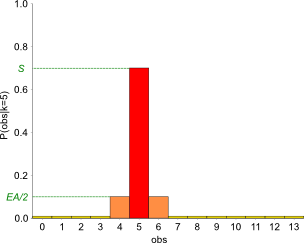
\includegraphics[scale=1.2]{obs_error.png}\\
\caption{Observation error probability distribution with a given true titre value. S = 0.7, EA = 0.2 and k = 5.}
\end{center}
\end{figure}


\item Interpretation: We infer posterior distributions for infection times for each individual independently, resulting in a 3036 univariate posterior distributions. With such sparse data, the inferred posterior distributions exhibit high amounts of uncertainty. To recover a point value for each parameter that might be indicative of infection, we take the proportion of estimates from the MCMC chain (post burn-in) that estimate an infection time, $ti$, before the second observation, t1. If the infection time estimate is between baseline and t1, then the data observed at t1 should reflect a boost. If an infection took place after the t1, then no true boost from that infection could possibly be observed (though there may be cross-reactive boosting). Therefore, estimates for $ti$ that come after t1 suggest that no infection took place. A high value for this proportion indicates that infection took place inbetween t0 and t1, whereas a low value suggests that no infection took place during the study.

\end{enumerate}

\section{Simulation Results}
An example output of the simulation framework using the parameters and protocol as desribed above is provided in an accompanying file: ``results.csv''. To summarise the above assumptions:

\begin{enumerate}
\item 1012 individuals, with sample times corresponding to the sample times from the FluScape data in days.
\item Three influenza strains.
\item All log titre levels at baseline are 0
\item Time-to-peak of 21 days for all boosts; waning rate of 0.002 log units per day; strong homologous boosting and some weak cross-reactive boosting.
\end{enumerate}

The columns in order are:
\begin{enumerate}
\item Individual ID
\item Time in days since baseline of first sample
\item Log titre readings for the three strains at t0
\item Time in days since baseline of the second sample
\item Log titre readings for the three strains at t1
\item Simulated infection times for each of the three strains in days since baseline. Note that a value of 912 suggests no infection, and any value greater than t1 for that individual would not be detected.
\item Inferred infection ``proportions'' for each of the three strains. That is, proportion of estimates in the MCMC chain that infer an infection time between baseline and t1.
\end{enumerate}

\newpage
\section{Example posteriors}
Below are a number of posterior distributions from the inference framework. I have taken 5 random individuals from the simulated serosurvey: individual 27, 282, 442, 464 and 672.

The model appears to be able to estimate the presence of absence of infection in a binary sense well, but the sparsity of the date makes inference on exact infection time very difficult.

\begin{figure}[H]
\begin{centering}
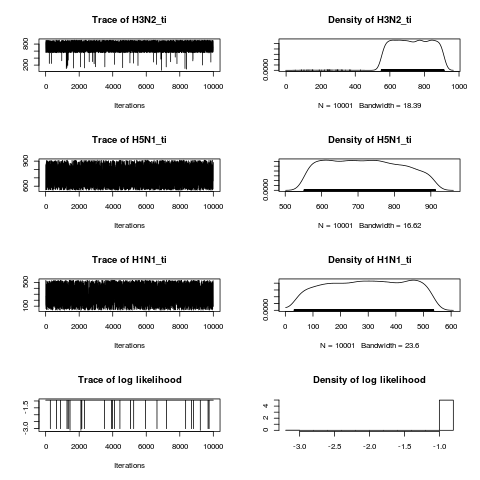
\includegraphics[scale=0.8]{27_mcmc.png}\\
\caption{Posterior distributions for individual 27. Actual infection times: 602 H3N2, 912 H5N1, 350 H1N1. t0 = 34 and t1 = 554. The model is able to predict the presence of H1N1 infection and the absence of H5N1/H3N2 infection}
\end{centering}
\end{figure}

\begin{figure}[H]
\begin{centering}
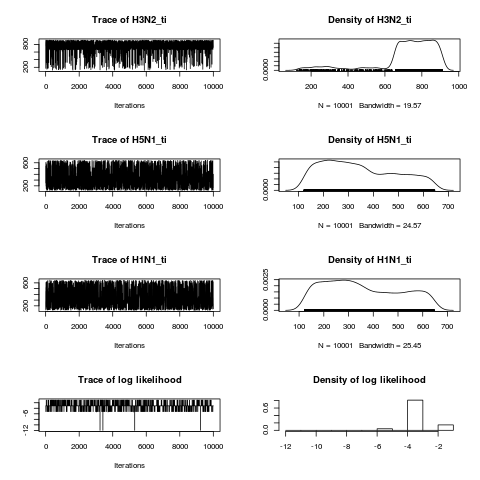
\includegraphics[scale=0.8]{282_mcmc.png}\\
\caption{Posterior distributions for individual 282. Actual infection times: 401 H3N2, 406 H5N1, 149 H1N1. t0 = 125 and 51 = 664. The model does not detect the H3N2 infection, as it is quickly overshadowed by the H5N1 infection. However, it does assign some probability to a definite H3N2 infection (~20\%)}
\end{centering}
\end{figure}

\begin{figure}[H]
\begin{centering}
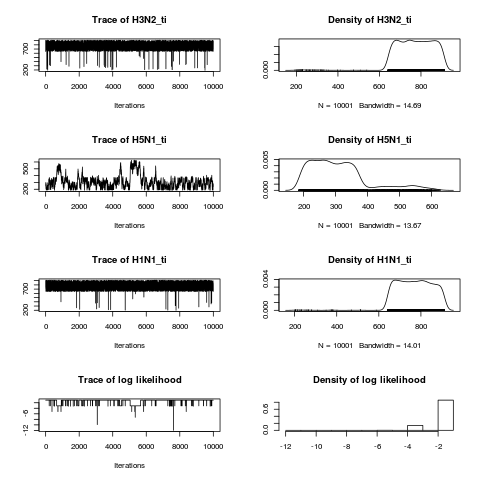
\includegraphics[scale=0.8]{442_mcmc.png}\\
\caption{Posterior distributions for individual 442. Actual infection times: 912 H3N2, 357 H5N1, 752 H1N1. t0 = 190 and t1 = 644. The model correctly estimates the presence the H5N1 infection and absence of H3N2/H1N1 infection}
\end{centering}
\end{figure}

\begin{figure}[H]
\begin{centering}
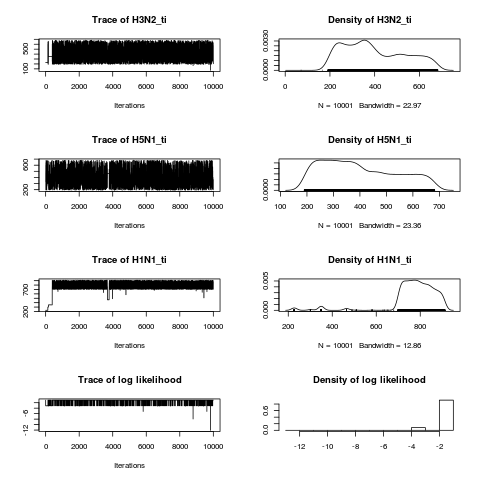
\includegraphics[scale=0.8]{464_mcmc.png}\\
\caption{Posterior distributions for individual 464. Actual infection times: 379 H3N2, 232 H5N1, 912 H1N1. t0 = 195 and 51 = 701. The model correctly estimates the presence of H3N2 and H5N1 infections, and the absence of H1N1 infection.}
\end{centering}
\end{figure}

\begin{figure}[H]
\begin{centering}
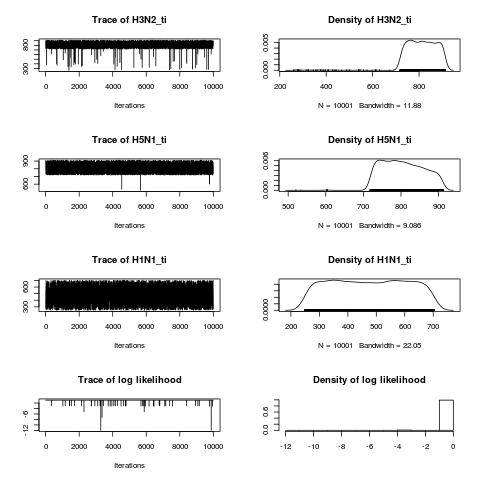
\includegraphics[scale=0.8]{672_mcmc.png}\\
\caption{Posterior distributions for individual 672. Actual infection times: 554 H3N2, 912 H5N1, 357 H1N1. t0 = 252 and t1 = 721. The model correctly estimates the presence of H1N1 infection, and the absence of H5N1/H3N2 infections.}
\end{centering}
\end{figure}

\newpage

\section{Further Work}
A few ideas:
\begin{enumerate}
\item Add observation error to the simulation.
\item Use t0 observations from FluScape data.
\item Quantify model sensitivity/specificity.
\item See how much better model predictions are with third time point, t2 (framework is set up to do this already).
\item Try different parameter values for boosting and waning. See how well model performs with higher cross-reactivity.
\item Incorporation of priors (ILI incidence).
\item Adapt framework to estimates population-wide boosting and waning parameters.
\item Stochastic process - eg. boosting drawn from a Poisson distribution.
\end{enumerate}


\section{Appendix}
\subsection{Model description}
Prior to the first infection, the log antibody titre value is likely to be 0. For each subsequent infection, initial antibody for a particular infecting strain, $k$, are given by:
\begin{equation}
 y_{0_{(k,j)}}=\left\{
 \begin{array}{lr}
   y_{0_{(k-1)}} & k \leqslant 1\\\\
   (\frac{\mu_{(k-1)}}{+tp_{(k-1)}}*(ti_k-ti_{(k-1)}) + y_{0_{(k-1)}} & ti_{(k)} \leqslant ti_{(k-1)} + tp_{(k-1)}\\\\
   m_{(k-1)}(ti_{(k-1)}+tp_{(k-1)}-ti_k)+\mu_{(k-1)} + y_{0_{(k-1)}}& else
 \end{array}
\right.
\end{equation}

Therefore, for an individual with an infection history of $(ti_k)_{(k=1)}^n$, where $n$ is the total number of infections and $ti_k$ is the time of infection with strain $k$, the kinetics of antibodies against strain $j$ are given by:

\begin{equation}
y(t, j) = \left\{
\begin{array}{lr}
y_{0_{(1,j)}} & t \leqslant ti_1\\\\
\frac{\mu_{(1,j)}}{tp_{(1,j)}}t-\frac{\mu_{(1,j)}}{tp_{(1,j)}}ti_1 + y_{0_{(1,j)}} & ti_1 < t \leqslant ti_1 + tp_{(1,j)}\\\\
-m_{(1,j)}t + m_{(1,j)}(ti_1+tp_{(1,j)})+\mu_{(1,j)}+y_{0_{(1,j)}} & ti_1+tp_{(1,j)} < t \leqslant ti_2\\\\
\frac{\mu_{(2,j)}}{tp_{(2,j)}}t-\frac{\mu_{(2,j)}}{tp_{(2,j)}}ti_2 + y_{0_{(2,j)}} & ti_2 < t \leqslant ti_2 + tp_{(2,j)}\\\\
-m_{(2,j)}t + m_{(2,j)}(ti_2+tp_{(2,j)})+\mu_{(2,j)}+y_{0_{(2,j)}} & ti_2+tp_{(2,j)} < t \leqslant ti_3\\\\
\vdots\\\\
\frac{\mu_{(n,j)}}{tp_{(n,j)}}t-\frac{\mu_{(n,j)}}{tp_{(n,j)}}ti_n + y_{0_{(n,j)}} & ti_n < t \leqslant ti_n + tp_{(n,j)}\\\\
-m_{(n,j)}t + m_{(n,j)}(ti_n+tp_{(n,j)})+\mu_{(n,j)}+y_{0_{(n,j)}} & ti_n+tp_{(n,j)} < t
\end{array}
\right.
\end{equation}

Where $y_{0_{(k,j)}}$ is the titre of antibodies against strain $j$ at the time of infection with strain $k$; $\mu_{(k,j)}$ is the level of boosting of antibodies to strain $j$ elicited following infection with strain $k$; $tp_{(k,j)}$ is the time at which this boost peaks; and $m_{(k,j)}$ is the rate at which is boost wanes.

As each strain potentially provides a cross-reactive boost to each other strain under consideration, it is helpful to think about each of these parameters as coming from an $n$ by $n$ matrix, where $n$ is the total number of strains under consideration.



\end{document}
